% !TEX root = ../main.tex

\section{introduction}
\label{sec:org662677c}


Many real-world classification problems are challenging because of
subjectivity issues, unclear (or overlapping) class-boundaries and
disagreement between annotators. For example, the movie \textit{Tenet} generated 
debates about which movie genre it belongs to, besides debates on content among the selected few who understood it. IMDB simultaneously categorizes it as \textit{action}
\textit{sci-fi} and \textit{thriller}. In a different domain, a seminal machine learning publication in which the authors propose to train with bigger batch sizes~\cite{bigBS} is categorized as \textit{Machine Learning (cs.LG)},
\textit{Computer Vision and Pattern Recognition (cs.CV)}, \textit{Distributed,
Parallel, and Cluster Computing (cs.DC)}, and \textit{Machine Learning
(stat.ML)} on \textit{arXiv}~\cite{bigBSArxiv}.

% \textit{Tenet} was a confusing movie. Aside from its complex content, debates are fusing about which movie genre it belongs to. IMDB categorizes it as \{\textit{action; sci-fi; thriller}\}. Also controversial, a seminal Machine Learning publication proposed training with bigger batch sizes as a general recommendation~\cite{bigBS} (the \#GreenAI movement later emerged to condemn delegating more computing power to neural networks at any environmental cost). This paper was categorized on Arxiv as \{\textit{Machine Learning (cs.LG); Computer Vision and Pattern Recognition (cs.CV); Distributed, Parallel, and Cluster Computing (cs.DC); Machine Learning (stat.ML)}\}. In cancer research, an ongoing discourse is concerned with categorizing cells' capabilities (e.g. \{\textit{resistance to immune system, enhanced proliferation}\}): at a certain point to be determined, cells have acquired enough of these capabilities to be malignant~\cite{cancerHallmarks}.

% These examples above in the domains of cinema and publication have several things in common. (I) Labels such as \textit{thriller} and \textit{machine learning} are abstract and debatable concepts to a certain degree (as opposed to \textit{featured actor x}, \textit{featured in journal x}) (II) The possibility of attributing more than one category to a single movie or a paper is desirable (i.e. labels are not mutually exclusive for the benefit of creativity / research). (III) The movie or paper as a whole needs to be looked at to categorize it. It requires an entire viewing of the movie \textit{Tenet} to determine if the label \textit{Romance} might not also be appropriate, as it is arguably the underlying driver of the protagonists. In other words, complex combinations of features in the movie are related to a label. In the contrary, it would be hard to isolate elements within these examples (such as a particular scene in a movie or a particular expression in a paper) as uniquely predictive of a single of their labels. (IV) The number of labels to attribute to each example is unknown at inference time.

The examples given above in the domains of cinema and publishing have several things in common: 
\begin{enumerate*}[label=(\arabic*)]
\item Labels such as \textit{thriller} and \textit{machine learning} are abstract and
debatable concepts to a certain degree (as opposed to \textit{featured actor
x}, \textit{featured in journal x}). 
\item The possibility of attributing more than one label to a single movie or a paper is desirable (i.e. labels are
mutually inclusive: one example can have more than one label). 
\item The movie or paper as a whole needs to be looked at to label it. It requires an entire
viewing of the movie \textit{Tenet} to determine if the label \textit{Romance}
might not also be appropriate, as it is arguably the underlying driver of the
protagonists. In other words, complex combinations of features in the movie
are related to a label. In the contrary, it would be hard to isolate elements
within these examples (such as a particular scene in a movie or a particular
expression in a paper) as uniquely predictive of a single of their labels.
\item The number of labels to attribute to each example is unknown at inference
time.
\end{enumerate*}


These four criteria do not appear together in a single problem definition in the existing literature, to the best of our knowledge. We thus propose to formalize the learning task of \textbf{F}ull-\textbf{I}nstance\textsuperscript{(III)} \textbf{M}ultilabel\textsuperscript{(II)} \textbf{P}rediction for \textbf{U}nknown\textsuperscript{(IV)} \textbf{L}abel counts (FIMPUL). [definitions and problem statement] + [this is common n IR]

% Regarding nomenclature, there seems to exist a consensus over the terms \emph{multiclass} and \emph{multilabel learning}, meaning mutually exclusive and non-mutually exclusive labels \footnote{non-mutually exclusive means here one example can have more than one label}, respectively~\cite{multilabelMethods}. Multilabel learning can therefore be seen as a subdomain of multiclass learning, where more than one class can be correct for the same example. We propose the term single-instance as opposed to multi-instance learning~\citep[e.g.,][]{multiInstance, multiInstanceMultiLabel}, for which it is considered natural to first segment an image / text / sound before performing prediction on each of the segments.

% That full/multi instance distinction helps explain why the abstract\textsuperscript{(I)} aspect can be considered implicit in FIMPUL. Beyond identifying object types (see YOLO \cite{YOLO} and its successors), performing face recognition (see FaceNet \cite{FaceNet} and its successors) on segments of an image, neural networks should soon be able to predict genres/categories of text, image and sound at high levels of accuracy. Neural network models are able to learn increasingly more abstract representations via deeper networks, representation learning and self-supervision~\citep[see, e.g.,][]{SS,Rep}. Hence, we would expect that they also get better at predicting more abstract labels. Towards this goal, there is a significant volume of recent work on building neural networks with a high-level of abstract understanding in the embedding space~\mdr{REF}. However, there seems\daan{vague} to be limited research on developing optimization frameworks that are adapted for these abstract concepts in the output space.

To solve multilabel tasks, existing optimization frameworks are still largely based on variations of the cross-entropy loss, with recently some advances in dealing with sparsity~\citep[see, e.g.,][]{focalLoss,tencent}. The existing measures to deal with FIMPUL can be divided into fit-data-to-algorithm (reverting back to a known problem formulation like multiclass unilabel classification) and fit-algorithm-to-data (adapting existing classification algorithms for the problem at hand). In the former case, cross-entropy losses are used at training time and thresholding is done at inference time. In the latter, elements of the learning algorithm are changed (such as the backpropagation procedure or the tasks). We propose a design-algorithm-for-data approach: [description here]

Machine learning prediction tasks' output are probabilistic (or a reversible transformation of a probabilistic measure such as a sigmoid or a soft max function). At training time, these probabilistic values are compared to binary values in the case of binary encoding of classes. At inference time, if the number $n_i$ of labels to be predicted per example is known a priori, it is natural to assign the $top_{n_i}$ predictions to that example~\cite{lossTopKError, topKmulticlassSVM}. If the number of labels per example is unknown a priori, the question remains at inference time as to how to extract information about the number of labels to assign to each example, aside from the propensity of labels to be assigned. This is generally done via a \emph{decision threshold}, that can be set globally for all examples. This threshold can optimize for specificity or sensitivity~\cite{decisionThreshold}. We propose a method where this threshold is implicitely defined, thanks to the use of metrics that already penalize for wrong label counts.

% \begin{figure}[t]
% \centering
% 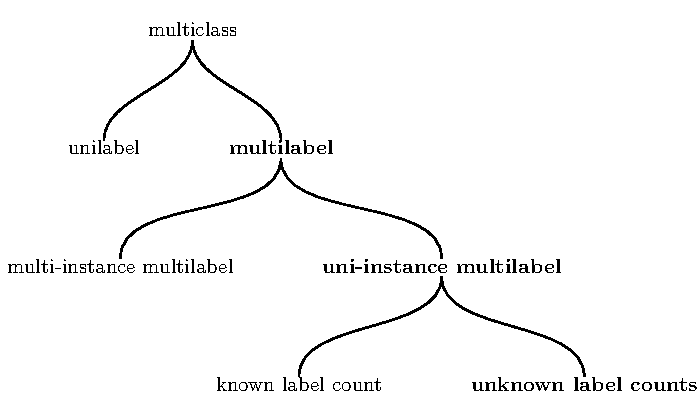
\includegraphics[width=.9\linewidth]{./tree/Tree.pdf}
% \caption{\label{fig:tree}
% FIMPUL (bold) within the \emph{multiclass} nomenclature
% % Clarifying ``multiclass'' classification problems.
% % In this paper we focus on the uni-instance, multilabel, multiclass classification problem with a varying number of labels (the bottom right hand side of the tree).
% }
% \end{figure}
% % \mdr{Image source ...}

Learning to Rank (the practice of using Machine Learning to sort documents according to their relevance) lead to the widespread use of certain metrics~\cite{LTR}. In a number of retrieval tasks, a model's out of sample accuracy is measured on metrics such as AUROC, F1 score, etc. These reflect an objective catered towards evaluating the model over an entire ranking. Due to the lack of differentiability, these metrics cannot be directly used as loss functions at training time (in-sample). A seminal study~\cite{optimizableLosses} derived a general framework for deriving decomposable surrogates to some of these metrics. We propose our own decomposable surrogates of classical confusion matrix metrics and in particular sigmoidF1 tailored for the problem at hand.

In this paper, we first propose a general mathematical formulation of FIMPUL tasks and thus place it within the multiclass nomenclature. The generalization encompasses different levels of complexity, from the classical cross-entropy loss up to the proposed loss function. \emph{sigmoidF1} is a F1 score surrogate, with a sigmoid function acting as a surrogate thresholding step function. This allows the use of the F1 metric which implicitly optimizes for label prediction and count simultaneously in a single task.  \emph{sigmoidF1} is benchmarked against loss functions commonly used in multiclass learning and other existing models that are closely related to the SIMPUL setting. We show that our custom losses improve predictions over the current state-of-the-art on several different metrics, across text (especially on the Arxiv dataset which, to the best of our knowledge, is the first use since its publication in August 2020) and image related tasks. We then conclude and propose future implementations for other labeling tasks.

% -----


% % \textbf{multi-class classification problems are hard}


% \paragraph{Problem statement}
% The examples given above in the domains of cinema and publishing have several things in common: 
% \begin{enumerate*}[label=(\arabic*)]
% \item Labels such as \textit{thriller} and \textit{machine learning} are abstract and
% debatable concepts to a certain degree (as opposed to \textit{featured actor
% x}, \textit{featured in journal x}). 
% \item The possibility of attributing more than one label to a single movie or a paper is desirable (i.e. labels are
% mutually inclusive: one example can have more than one label). 
% \item The movie or paper as a whole needs to be looked at to label it. It requires an entire
% viewing of the movie \textit{Tenet} to determine if the label \textit{Romance}
% might not also be appropriate, as it is arguably the underlying driver of the
% protagonists. In other words, complex combinations of features in the movie
% are related to a label. In the contrary, it would be hard to isolate elements
% within these examples (such as a particular scene in a movie or a particular
% expression in a paper) as uniquely predictive of a single of their labels.
% \item The number of labels to attribute to each example is unknown at inference
% time.
% \end{enumerate*}

% In this paper we focus on such learning problems,  which we call \emph{Single-Instance Multilabel Prediction
% for Unknown Label counts} (SIMPUL).
% More precisely, 
% \begin{itemize}
% \item \mdr{It's good to have a sharp definition of the problem space, whether it is SIMPUL or something else. And no, we do not need to sell it, we just need to identify it in a precise manner.}
% \item \mdr{a CONCISE definition of the problem, like in the paper by \citet{multilabelMethods}; no discussion, just definition.}
% \item \mdr{NO DISCUSSION, just a concise statement}
% \item \mdr{Include a comment that SIMPUL problems are very common in IR, as we sho in the related work sectino below.}
% \end{itemize}

% \paragraph{Optimization frameworks to SIMPUL}
% As we explain in Section~\ref{section:background}, previous optimization frameworks for SIMPUL problems come in two flavors. 
% \begin{itemize}
% \item flavor  1
% \item flavor 2
% \end{itemize}
% We introduce a new flavor, 
% \begin{itemize}
% \item Why? One sentence about what's wrong with flavors 1 and 2
% \item Bring in the idea of confusion matrix metrics, etc. Just two sentences. No abstract stuff.
% \item What? One sentence about The New Thing.
% \end{itemize}

% \paragraph{Contributions}
% In this paper, we first propose a class of smooth loss functions that optimize
% learning in SIMPUL problems. 
% \mdr{What does this mean? The generalization encompasses different levels
% of complexity, from the classical cross-entropy loss up to the proposed loss
% function.} 
% \mdr{Isn't this too specific for the introduction; you haven't introduced this; how does it connect to confusion matrix metrics: We propose the \emph{sigmoidF1}: an F1 score surrogate, with a sigmoid function acting as a surrogate thresholding step function.} This allows for
% the use of the F1 metric which implicitly optimizes for label prediction and
% count simultaneously in a single task and is robust to outliers.
% \emph{sigmoidF1} and its adaptive \emph{SadF1} and Bayesian \emph{SBayesF1}
% counterparts are benchmarked against loss functions commonly used in
% multiclass learning and other existing models that are closely related to the
% SIMPUL setting. 

% We show that our custom losses improve predictions over the
% current  state-of-the-art on several different metrics, across text
% (especially on the arXiv dataset which, to the best of our knowledge, is the
% first use since its publication in August 2020) and image related tasks.

% \paragraph{The remainder of the paper}
% The remainder of this paper is structured as follows: first, we introduce
% our method and define a class of smooth loss functions for SIMPUL problems.
% Next, we detail our experimental setup and describe the datasets used in our
% experiments. After presenting the experimental results in the next section,
% we close the paper with conclusions and propositions for future work.


% %%% Local Variables: %% mode: latex %% TeX-master: "../main" %% End:
